\documentclass[aspectratio=169]{beamer}

\usepackage{amsmath, amssymb, amsxtra, amsthm, amsfonts}
\usetheme{moloch}
\usecolortheme{beaver}
\setbeamertemplate{footline}
{
  \leavevmode%
  \hbox{%
    \begin{beamercolorbox}[wd=.5\paperwidth,ht=2.25ex,dp=1ex,center]{author in head/foot}%
      \usebeamerfont{author in head/foot}\insertsection
    \end{beamercolorbox}%
    \begin{beamercolorbox}[wd=.5\paperwidth,ht=2.25ex,dp=1ex,right]{date in head/foot}%
      \usebeamerfont{date in head/foot}\inserttitle\hspace*{2em}
      \insertframenumber{} / \inserttotalframenumber\hspace*{2ex}
    \end{beamercolorbox}}%
  \vskip0pt%
}
\makeatother

\usepackage[english]{babel}
\usefonttheme{serif}

\usepackage{mathtools}
\usepackage{graphicx}
\usepackage{bm}
\usepackage{color}
\usepackage[dvipsnames,table]{xcolor}
\usepackage{tikz}
\usepackage{stanli}
\usepackage{verbatim}
\usepackage{tikz}
\usetikzlibrary{shapes,calc,through,3d,patterns}
\usetikzlibrary{decorations.pathreplacing}
\usetikzlibrary{arrows.meta,calc,positioning}

\usepackage{pgfplots}
\usepackage{siunitx} % For formatting numbers
\usepackage{hyperref}
\hypersetup{colorlinks=true,linkcolor=darkred}
\usepackage{multicol}
\usepackage[absolute,overlay,]{textpos}
\usepackage{pgfplots}
\pgfplotsset{width=10cm,compat=1.9}
\usepackage{subcaption}
\usepackage{multirow}
\usepackage{bbding}
\usepackage{arydshln}
\usepackage{mathtools}
\usepackage{tcolorbox}
\usepackage{animate}

\textblockorigin{80mm}{45mm}


\newtheorem{thm}{Theorem}
\newtheorem{cor}[thm]{Corollary}
\newtheorem{prop}[thm]{Proposition}
\newtheorem{lem}[thm]{Lemma}
\theoremstyle{remark}
\newtheorem*{rem}{Remark}

%Block def
\definecolor{darkred}{rgb}{0.6,0,0}
\setbeamertemplate{blocks}[rounded][shadow=false]
\setbeamercolor{block title}{bg=darkred!15,fg=black}
\setbeamercolor{block body}{bg=darkred!5,fg=black}

\setbeamercolor{itemize item}{fg=darkred}
\setbeamercolor{itemize subitem}{fg=darkred}
\setbeamercolor{itemize subsubitem}{fg=darkred}
\setbeamercolor{enumerate item}{fg=darkred}
\setbeamercolor{button}{bg=gray!30,fg=darkred}

\setbeamertemplate{itemize item}[square]
\setbeamertemplate{itemize subitem}[circle]
\setbeamertemplate{itemize subsubitem}[triangle]
\setbeamertemplate{enumerate items}[circle]
\setbeamercolor{item projected}{bg=darkred}

\newcommand{\bolddelta}{\boldsymbol\delta}
\newcommand{\boldxi}{\boldsymbol\xi}
\DeclareMathOperator*{\A}{\text{\raisebox{-0.2cm}{\Huge A}}}




\title{Dynamic analysis of beams, frames and grids}
\subtitle{Special structural elements}
\author{ME473 Dynamic finite element analysis of structures}
\institute{Stefano Burzio}
\date{2025}

\begin{document}
\usenavigationsymbolstemplate{}

\section{Geometric stiffness}

\begin{frame}{Beam subjected to axial loads}
  \begin{itemize}
    \item Consider a beam subjected to axial forces $N$ applied at both ends.
  \end{itemize}
  \begin{center}
    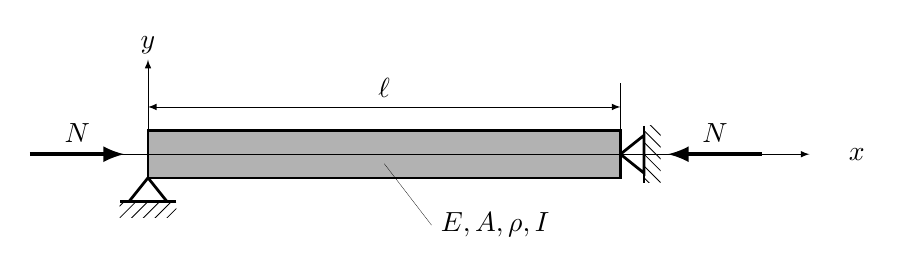
\begin{tikzpicture}[scale=0.6]
      \point{a}{0}{0};
      \point{b}{6}{0.5*0.6};
      \support {1}{a}[0];
      \support {1}{b}[90];
      % Draw the rectangle
      \filldraw[fill=gray!60, draw=black,thick] (0,0) rectangle (10,1);
      %axis
      \draw[-latex, ultra thin] (-1,0.5) -- (14,0.5);
      \draw[-latex, ultra thin] (0,0) -- (0,2.5);
      \node at (15,0.5) {\(x\)};
      \node at (0,2.8) {\(y\)};
      % length
      \draw[ultra thin] (10,0) -- (10, 2) ;
      \draw[latex-latex, ultra thin]  (0,1.5)  to node[sloped,midway,above] {$\ell$}(10,1.5) ;
      % N
      \draw[latex-, ultra thick] (11,0.5) -- (13,0.5) node[midway, above]{$N$};
      \draw[-latex, ultra thick] (-2.5,0.5) -- (-0.5,0.5) node[midway, above]{$N$};
      \draw[ultra thin]  (5,0.3) -- (6,-1) node[right]{$E,A,\rho,I$};
    \end{tikzpicture}
  \end{center}
  \begin{itemize}
    \item Beam carrying large axial loads or undergoing large displacements have nonlinear behavior arising from the internal moments that are the product of the axial loads and the displacements transverse to the loads.
    \item The stiffness coefficients $k_{ij}$ must be modified by the presence of the axial force to the corresponding \textbf{geometric stiffness coefficients} $k^g_{ij}$.
  \end{itemize}
\end{frame}

\begin{comment}
\begin{frame}{Geometric stiffness matrix}
  \begin{block}{}
    For frame elements with transverse rotation $\theta_3(x,t)$, but without displacements along the axial coordinate $x$ the frame element undergoes axial deformation $u_1(x,t)$.
  \end{block}
  \vspace{0.3cm}
  \begin{columns}
    \begin{column}{.45\textwidth}
      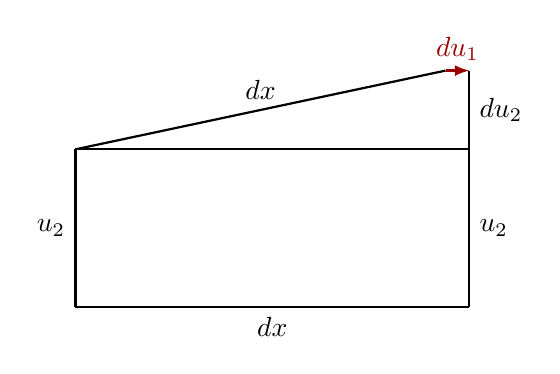
\begin{tikzpicture}
        \draw[thick] (0,0) -- (5,0) node[midway, below]{$dx$};
        \draw[thick] (5,0) -- (5,2) node[midway, right]{$u_2$};
        \draw[thick] (5,2) -- (5,3) node[midway, right]{$du_2$};
        \draw[thick] (0,0) -- (0,2) node[midway, left]{$u_2$};
        \draw[thick] (0,2) -- (5,2);
        \draw[thick] (0,2) -- (4.7,3) node[midway, above]{$dx$};
        \draw[thick,-latex,darkred] (4.7,3) -- (5,3) node[midway, above]{$du_1$};
      \end{tikzpicture}    \end{column}
    \begin{column}{.45\textwidth}
      Using the Pythagorean theorem:
      $$dx^2=(dx-du_1)^2+du_2^2$$
      $$\frac{du_1}{dx}=\frac{1}{2}\left(\frac{du_1}{dx}\right)^2+\frac{1}{2}\left(\frac{du_2}{dx}\right)^2$$
      Axial strain is less than transverse rotations:
      $$\frac{du_1}{dx}\approx \frac{1}{2}\left(\frac{du_2}{dx}\right)^2$$
    \end{column}
  \end{columns}
\end{frame}


\begin{frame}{Geometric stiffness matrix}
  \begin{itemize}
    \item Strain energy associated with axial forces $N(x)$ and axial geometric deformation
          \[
            U_G = \int_0^\ell N(x) \frac{du_1(x)}{dx} \, dx = \frac{1}{2} \int_0^L N(x) \left( \frac{du_2(x)}{dx} \right)^2 dx.
          \]
    \item Employing the approximation $u_2^h(x,t)=\mathbf H(x)\mathbf q(t)$ yield to
          \[
            U_G = \frac{1}{2} \mathbf q^T\int_0^L N(x) \frac{d\mathbf H}{dx}^T\frac{d\mathbf H}{dx}\,  dx \ \mathbf q.
          \]
    \item The geometric stiffness matrix is defined as
          $$\mathbf K^g=\int_0^\ell N(x)\, \frac{d\mathbf H}{dx}^T\frac{d\mathbf H}{dx}\ dx$$
  \end{itemize}
\end{frame}
\end{comment}

\begin{frame}{Geometric stiffness matrix}
  \begin{block}{}
    $k^g_{ij}$ is defined as the force corresponding to the nodal coordinate $i$ due to a unit displacement at coordinate $j$ and resulting for the axial force $N$.
  \end{block}
  \textbf{Calculation of $k^g_{12}$}: vertical force at node 1 due to a unit rotation $\theta_2=1$ caused by the axial force $N$. May be evaluated by the principle of virtual work:
  \vspace{0.3cm}
  \begin{columns}
    \begin{column}{.45\textwidth}
      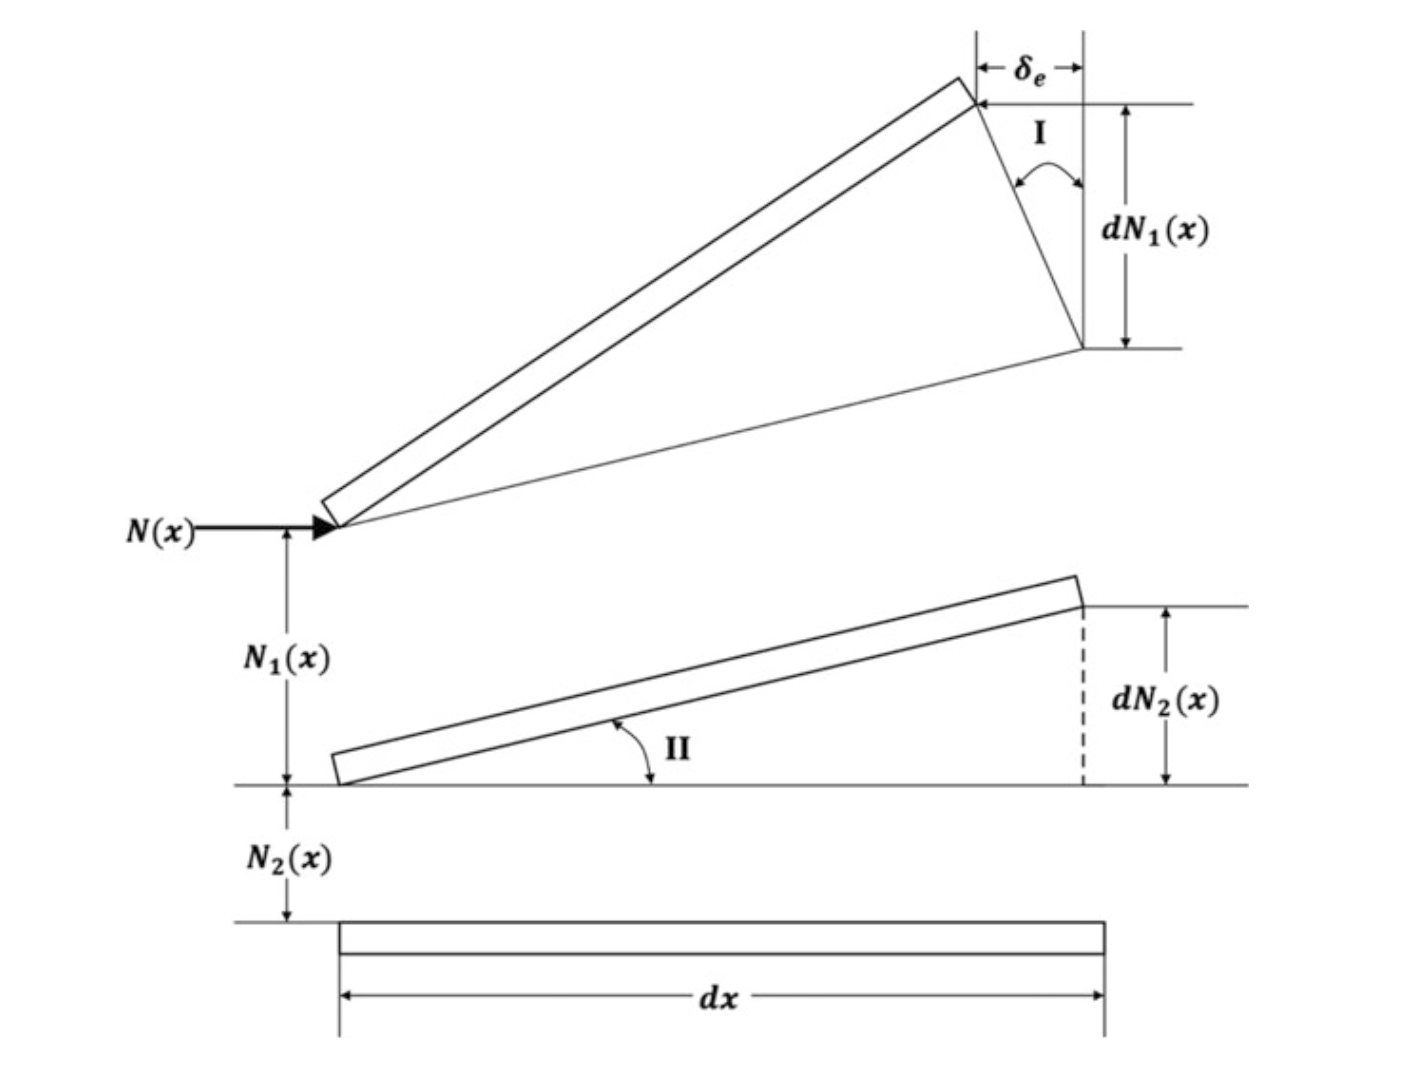
\includegraphics[width=4.5cm]{../images/geometricStiffness.png}
    \end{column}
    \begin{column}{.45\textwidth}
      $$dW=N\delta_e$$
      By similar triangles we have
      \begin{align*}
        \frac{\delta_e}{dh_1(x)} & =\frac{dh_2(x)}{dx}                         \\
        \delta_e                 & = \frac{dh_1}{dx}(x)\frac{dh_2}{dx}(x)\, dx
      \end{align*}
    \end{column}
  \end{columns}
  $$k^g_{12}=N\int_0^\ell h_1^\prime(x)h_2^\prime(x)\, dx$$
\end{frame}

\begin{frame}{Geometric stiffness matrix}
  \begin{itemize}
    \item In general, any geometric stiffness coefficient may be expressed as
          $$k^g_{ij}=N \int_0^\ell h_i^\prime(x)h_i^\prime(x)\, dx$$
    \item We define the \textbf{geometric stiffness matrix} as:
          $$\mathbf K^g=N\int_0^\ell \, \frac{d\mathbf H}{dx}^T\frac{d\mathbf H}{dx}\ dx$$
    \item When $N$ is constant along the beam length we obtain
          $$\mathbf K^g=\frac{N}{30\ell}\begin{bmatrix}
              36    & 3\ell   & -36    & 3\ell   \\
              3\ell & 4\ell^2 & -3\ell & -\ell^2 \\
              -36   & -3\ell  & 36     & -3\ell  \\
              3\ell & -\ell^2 & -3\ell & 4\ell^2 \\
            \end{bmatrix}
          $$
  \end{itemize}
\end{frame}

\begin{frame}{Example: stability of Bernoulli beam}
  \begin{center}
    \href{https://drive.mathworks.com/sharing/6a9792ef-d0a7-4aca-a1d0-8b1862b0ac3b}{\beamergotobutton{Go to Matlab Drive}}
  \end{center}
\end{frame}

\end{document}